\documentclass[12pt,a4paper,ngerman,plainfootsepline,plainheadsepline]{scrreprt}
% Change "article" to "report" to get rid of page number on title page
\usepackage{amsmath,amsfonts,amsthm,amssymb}
\usepackage{setspace}
\usepackage{Tabbing}
\usepackage{lastpage}
\usepackage{cite}
\usepackage{tocbasic}
\usepackage[automark,						%Automatische Kopfzeile
						%headtopline,				%Linie über dem Seitenkopf
						%plainheadtopline,	%Plain, Linie über dem Seitenkopf
						headsepline,				%Linie zwischen Kopf und Textkörper
						%plainheadsepline,	%Plain, Linie zwischen Kopf und Textkörper
						footsepline,				%Linie zwischen Textkörper und Fuß
						plainfootsepline,   %Plain, Linie zwischen Textkörper und Fuß
						%footbotline,				%Linie unter dem Fuß
						%plainfootbotline   %Plain, Linie unter dem Fuß
						]{scrpage2}
\usepackage{graphicx,wrapfig}
%\usepackage[ansinew]{inputenc}
\usepackage{lmodern}
\usepackage{scrpage2}
\usepackage[utf8]{inputenc}
\usepackage[ngerman]{babel}
\usepackage{url}
\usepackage{fouriernc}
%\usepackage[scaled]{helvet}
\renewcommand*\familydefault{\sfdefault} %% Only if the base font of the document is to be sans serif
%\usepackage[T1]{fontenc}
% In case you need to adjust margins:
\topmargin=-0.45in      %
\evensidemargin=0in     %
\oddsidemargin=0in      %
\textwidth=6.5in        %
\textheight=9.0in       %
\headsep=0.25in         %
\setcounter{secnumdepth}{3}
\setcounter{tocdepth}{3}

% Homework Specific Information
\newcommand{\hmwkTitle}{Netzwerksicherheit}
\newcommand{\hmwkClass}{Handout}
\newcommand{\hmwkAuthorName}{Raphael Marques}

                                   %
\clearscrplain		
%Alte Plain-Formatierung entfernen
\clearscrheadfoot
\cehead{\hmwkClass}    % Chapter auf geraden Seiten (links) in Kopfzeile
\cohead{\hmwkClass}
\rehead{\includegraphics[width=25pt]{graphicszhaw.jpgg}}    % Logo auf geraden Seiten (rechts) in Kopfzeile
\rohead{
\includegraphics[width=25pt]{graphics/zhaw.jpg}}   % Logo auf ungeraden Seiten (links) in Kopfzeile
\lehead{\hmwkTitle}    % Section auf geraden Seiten (rechts) in Kopfzeile
\lohead{\hmwkTitle} 

\refoot{\hmwkAuthorName}    % Chapter auf geraden Seiten (links) in Kopfzeile
\rofoot{\hmwkAuthorName}
%\rofoot{Seite\ \thepage\ von\ \pageref{LastPage}}    % Chaper auf geraden Seiten (links) in Kopfzeile
%\refoot{Seite\ \thepage\ von\ \pageref{LastPage}}
\setheadsepline{0.4pt}   
\setfootsepline{0.4pt}                                  %
\pagestyle{scrheadings}
\automark[chapter]{chapter}
 % Seitenstil aktivieren
%\renewcommand{\chapterpagestyle}{scrheadings}
% This is used to trace down (pin point) problems
% in latexing a document:
%\tracingall


%%%%%%%%%%%%%%%%%%%%%%%%%%%%%%%%%%%%%%%%%%%%%%%%%%%%%%%%%%%%%
% Make title
%\title{\vspace{2in}\textmd{\textbf{\ \hmwkTitle}}\\\normalsize\vspace{0.1in}\large{\hmwkClass}\\\vspace{0.1in}\large{\textit{}}\vspace{3in}}

%\author{\textbf{\hmwkAuthorName}}
%\author{\textbf{Miro Ljubicic}\\ljubimir@students.zhaw.ch}
%%%%%%%%%%%%%%%%%%%%%%%%%%%%%%%%%%%%%%%%%%%%%%%%%%%%%%%%%%%%%
\begin{document}
\begin{spacing}{1.1}
%
%\maketitle
%\newpage
%% Uncomment the \tableofcontents and \newpage lines to get a Contents page
%% Uncomment the \setcounter line as well if you do NOT want subsections
%%       listed in Contents
%%\setcounter{tocdepth}{1}
%%\tableofcontents
%%\newpage
%
%% When problems are long, it may be desirable to put a \newpage or a
%% \clearpage before each homeworkProblem environment
%
%\clearpage
%\begin{normalsize}
%\setcounter{tocdepth}{2}
%\tableofcontents
%\end{normalsize}
\section*{Racketsports Manager}
Die Semesterarbeit erstellte einen Proof of Concept einer Applikation, mit welcher man verschiedene Anwendungsfälle rund um den Racketsport vereinfachen kann. Die Applikation will dem Benutzer helfen, andere Personen im geografischen Umfeld zu finden, einfach mit anderen Benutzern Termine zu vereinbaren, gespielte Spiele zu protokollieren sowie eine Liga zu managen. Die verschiedenen implementierten Benutzerfälle sind auf den Racketsport zugeschnitten.

Um die Anwendungsfälle zu implementieren, wurden eine Marktanalyse und eine Anforderungsanalyse erstellt, welche zu spezifischen Anforderungen führten. Nach einer Konzeption der Applikation und Auswahl der optimalen Technologien wurden die definierten Anforderungen implementiert und getestet. 

Die Applikation ist möglichst offen aufgebaut. Auf dem Server ist ein NodeJS MVC Framework --- ExpressJS --- in Operation, welches dem Client eine JSON API anbietet. Der Client ist eine AngularJS Applikation, welche den Inhalt bei der API bezieht und für den User in einem Browser oder einer Android Applikation anzeigt. Als Datenbank kommt MongoDB zum Einsatz, welche das JSON-Objekt speichert. Dieses wird ohne Konvertierungen bis zum Client geschickt und von diesem angezeigt.  Durch das Applikations-Design ist es möglich, viele andere Clients zu entwickeln, da alle Funktionen über die API verfügbar sind. Durch das MVC Framework sind die Funktionen gut voneinander entkoppelt und eine Erweiterung der Funktionalität ist unkompliziert. Für jeden Controller und jedes Model gibt es zusätzlich Unit-Tests, welche sicherstellen, dass alle Funktionen weiterhin korrekt funktionieren. 

Die Identifizierung von Personen im geografischen Umfeld wird durch die Racket-Sportzentren, in welchen bevorzugt gespielt wird, vollzogen. Dem Benutzer wird eine Liste gezeigt, welche anderen Spieler im gleichen Racket-Sportzentrum spielen. So ist es möglich, unkompliziert andere Spieler herauszufordern, ohne sie zu kennen. Termine sollen einfach, über einen Doodle ähnlichen Algorithmus, gefunden werden. Der Spieler, welcher das Spiel initiiert, kann mehrere Termine vorschlagen, während der andere Spieler Termine von den vorgeschlagenen Terminen auswählen kann. Um Spiele zu protokollieren, gibt es eine intuitive Eingabemaske, welche die Racketsport-typischen Sätze unterstützt. Diese Spiele können auch als Ligaspiel bezeichnet werden und werden somit direkt bewertet und in die Liga-Rangliste miteinbezogen.  Das Liga-Management bietet einen innovativen Auto-Herausforderungs-Mechanismus, bei welchem die Spieler jede  oder jede zweite Woche gegenseitig zu einem Spiel herausgefordert werden. Zusätzlich gibt es auch ein Punktesystem mit Rangliste, bei dem gespielte Matches zur Liga zählen. Zusätzlich bietet die Applikation ein Freunde-System, um mit neu kennengelernten Spielern in Kontakt zu bleiben und neue Spiele zu vereinbaren. 

Die Applikation beinhaltet die Objekte Racket-Sportzentrum, Spiel, Liga und User. Diese Objekte repräsentieren Elemente, um die Anwendungsfälle zu erfüllen. Das Racketsport-Zentrum-Objekt bietet dem Benutzer eine Liste von allen Spielern, welche auch in diesem Racket-Sportzentrum spielen, um so neue Spieler herauszufordern. Die Liga bietet eine Rangliste und einen Scheduling-Algorithmus, damit die Spieler der Liga regelmässig spielen gehen. Das Spiel bietet einen komplexen Terminvereinbarungs- und Protokollierungs-Algorithmus, damit alles fair abläuft. Beide Spieler haben immer die Möglichkeit, das Resultat zu korrigieren oder den Termin neu zu vereinbaren. 
%\input{subdoc/Glossar}
%\input{subdoc/Einleitung}
%\section{Grundlagen}

\subsection{Warum Identity Management}
\frame{\frametitle{Warum Identity Management}

\begin{center}
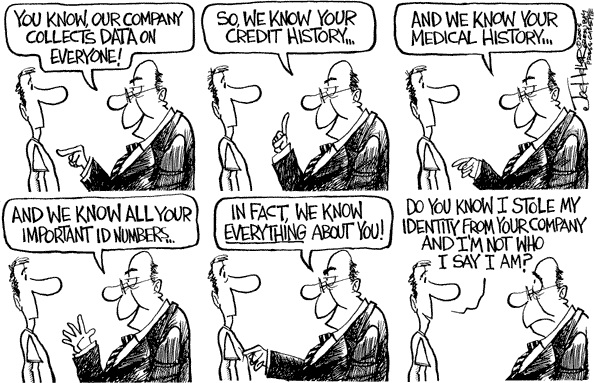
\includegraphics[scale=0.6]{pic/heller}
\end{center}

}

\frame{\frametitle{Warum Identity Management}

\begin{itemize}
\item Komplexer und wichtiger werdende IT Systeme
\item Steigende (digitale) Wirtschaftsspionage
\item Gesetzliche Anforderungen an den Datenschutz
\item Zeitdruck durch globale Wirtschaft und Konkurrenz
\end{itemize}

}

\subsection{Definitionen}

\subsubsection{Identität}
\frame{\frametitle{Identität}

\begin{shadequote}
Identität ist die Summe derjenigen Merkmale, anhand derer ein Individuum von anderen unterschieden werden kann.
\end{shadequote}

Wir beschränken wir uns auf die Merkmale welche digital erfassbar sind. Dazu zählen
ebenfalls gängige biometrische Verfahren.
}

\subsubsection{User}
\frame{\frametitle{User}
Hierbei handelt es sich in erster Linie um einen Menschen, welcher zum Sinne seiner Aufgabenerfüllung ein IT System nutzt. Es kann sich auch um einen \emph{virtuellen User} handeln. Dies ist der Fall wenn ein Programm über Rechte verfügt über welche es auf Ressourcen im Netzwerk zugreifen kann.
}

\subsubsection{Identity Management}
\frame{\frametitle{Identity Management}
Ist die Summe aller Maßnahmen, welche notwendig sind um einen User, eines IT Systems, eindeutig zu erkennen und ihn mit den entsprechenden Rechten zu versorgen, damit er seine Aufgaben ausführen kann. Alle diese Maßnahmen werden über standardisierte, nachvollziehbare Prozesse geregelt.
}

\subsubsection{Komplexität \& Zeit}
\frame{\frametitle{Komplexität \& Zeit}
Hierbei handelt es sich um die wichtigsten Faktoren welche das Identity Management beeinflussen. Die Komplexität bildet das benutzte IT System und das Betriebsorganigramm ab. Der Grad der Komplexität ist schon bei KMU recht hoch und wächst scheinbar exponentiell mit der Betriebsgröße. Zeit ist ein weiterer nicht zu unterschätzender Faktor, diese muss von zwei Seiten betrachtet werden. Zum einen muss das Identity Management in der Lage sein schnell auf eventuelle Änderungen bei den Usern zu reagieren. Zum anderen darf natürlich die Überprüfung der User Identität nicht zu viel seiner produktiven Zeit in Anspruch nehmen.
}
%\input{subdoc/ISO_IEC_20000}
%\input{subdoc/Umsetzung_Praxis}
%\input{subdoc/Prozessbeispiel_Incident}
%\input{subdoc/Weiterer_Ausblick}
%\input{subdoc/Fazit}
%\input{subdoc/Anhang_A}
%\listoffigures
%\nocite{*} 
%\bibliography{bib/bib1}{}
%\bibliographystyle{plain}
%%\bibliographystyle{alphadin}
%%\bibliographystyle{plain}
\end{spacing}
\end{document}